% Этот текст можно свободно редактировать.
\FloatBarrier
\section{Автоматизация признаков}

Идея связана с \href{https://groups.csail.mit.edu/EVO-DesignOpt/groupWebSite/uploads/Site/DSAA_DSM_2015.pdf}{Deep Feature Synthesis}: задать допустимые отношения и операции и автоматически проверять полученные признаки. Здесь реализована собственная небольшая грамматика с обязательной временной границей. Это не заявление о принципиально новом алгоритме и не свободный SQL-поиск агентом.

Грамматика расширяет ручной набор:

\begin{enumerate}
\item Окна \textbf{1, 3, 10, 14, 60 дней} для шести отношений, counts и условные доли.
\item Экспоненциальное забывание с half-life \(h\in\{2,10,30\}\) дней:
\begin{equation}
f_h(t)=\sum_{e:\,t_e<t}2^{-(t-t_e)/h},
\end{equation}
где \(t_e\) --- дата прошлого события. Выбираются формы памяти, а не только ширина жёсткого окна.
\item Тренды \code{(count_7/7)/(count_30/30+0.1)}.
\item Популярность объекта внутри возрастного сегмента за 7/30 дней и всю историю.
\item Сходство по всем жанрам: Jaccard с последним объектом и средняя/максимальная доля жанров кандидата в 30-дневной истории пользователя. При нескольких последних объектах одного дня выбор детерминирован по ID; это техническая договорённость при отсутствии внутридневного порядка.
\end{enumerate}
Весь банк содержит \textbf{128 признаков}, дополнительные признаки разбиты на \textbf{11 групп}. Сначала автоматически оценивается добавление каждой группы к ручному набору с бюджетом 180 деревьев; затем проверяются объединения лучших двух и трёх групп. Контрольная ручная модель обучается с тем же сокращённым бюджетом. Выбирается максимум NDCG@10 на search с порогом прироста 0.0005. Число групп ограничено 3; при равенстве выбирается более простой набор. После этого выбранный набор обучается с полным бюджетом. Подтверждающая валидация не участвует в генерации новых признаков.

Выбраны группы: \textbf{decay\_2d, window\_3d, window\_1d}. Итоговый набор: \textbf{74 признаков}. По confirm рекомендован вариант \textbf{automatic}. Все проверенные варианты и значения метрик сохранены в \code{search_log.json}, полный машинный реестр --- \code{feature_registry.json}.

\FloatBarrier
\begingroup
\setlength{\tabcolsep}{3pt}
\setlength{\reporttablewidth}{\dimexpr\linewidth-12pt\relax}
\renewcommand{\arraystretch}{1.15}
\small
\begin{longtable}{@{}>{\raggedright\arraybackslash}p{0.30457\reporttablewidth}>{\raggedright\arraybackslash}p{0.39086\reporttablewidth}>{\raggedright\arraybackslash}p{0.30457\reporttablewidth}@{}}
\caption{Автоматизация признаков}\label{tab:results-3}\\
\toprule
\textbf{Модель} & \textbf{Среднее NDCG@10 confirm по seed} & \textbf{SD} \\
\midrule
\endfirsthead
\multicolumn{3}{l}{\small\itshape Продолжение таблицы \thetable}\\
\toprule
\textbf{Модель} & \textbf{Среднее NDCG@10 confirm по seed} & \textbf{SD} \\
\midrule
\endhead
\midrule
\multicolumn{3}{r}{\footnotesize Продолжение на следующей странице}\\
\endfoot
\bottomrule
\endlastfoot
Ручные признаки & 0.48917 & 0.00181 \\
Автоотбор & 0.50258 & 0.00051 \\
\end{longtable}
\endgroup

Здесь показаны средние отдельных моделей, которыми принимается подтверждающее решение. Это отдельный период, не использованный для перебора групп. Ансамблевая метрика ниже относится к тесту.

\FloatBarrier
\begingroup
\setlength{\tabcolsep}{3pt}
\setlength{\reporttablewidth}{\dimexpr\linewidth-12pt\relax}
\renewcommand{\arraystretch}{1.15}
\small
\begin{longtable}{@{}>{\raggedright\arraybackslash}p{0.30489\reporttablewidth}>{\raggedright\arraybackslash}p{0.30113\reporttablewidth}>{\raggedright\arraybackslash}p{0.39398\reporttablewidth}@{}}
\caption{Автоматизация признаков}\label{tab:results-4}\\
\toprule
\textbf{Добавленная группа} & \textbf{NDCG@10 search} & \textbf{\ensuremath{\Delta} к контролю с тем же бюджетом} \\
\midrule
\endfirsthead
\multicolumn{3}{l}{\small\itshape Продолжение таблицы \thetable}\\
\toprule
\textbf{Добавленная группа} & \textbf{NDCG@10 search} & \textbf{\ensuremath{\Delta} к контролю с тем же бюджетом} \\
\midrule
\endhead
\midrule
\multicolumn{3}{r}{\footnotesize Продолжение на следующей странице}\\
\endfoot
\bottomrule
\endlastfoot
decay\_2d & 0.50535 & +0.01132 \\
window\_3d & 0.50524 & +0.01122 \\
window\_1d & 0.50403 & +0.01001 \\
multigenre & 0.50228 & +0.00826 \\
trends & 0.50176 & +0.00774 \\
window\_60d & 0.49601 & +0.00199 \\
segment & 0.49548 & +0.00145 \\
decay\_10d & 0.49533 & +0.00131 \\
window\_14d & 0.49452 & +0.00050 \\
window\_10d & 0.49450 & +0.00048 \\
decay\_30d & 0.49383 & -0.00019 \\
\end{longtable}
\endgroup

Лучший одиночный шаг на search --- \code{decay_2d}; его выигрыш +0.01132. Самый слабый шаг --- \code{decay_30d}, изменение -0.00019. Это оценка полезности в процессе поиска, а не независимые тестовые эффекты.

\begin{figure}[!htbp]
\centering
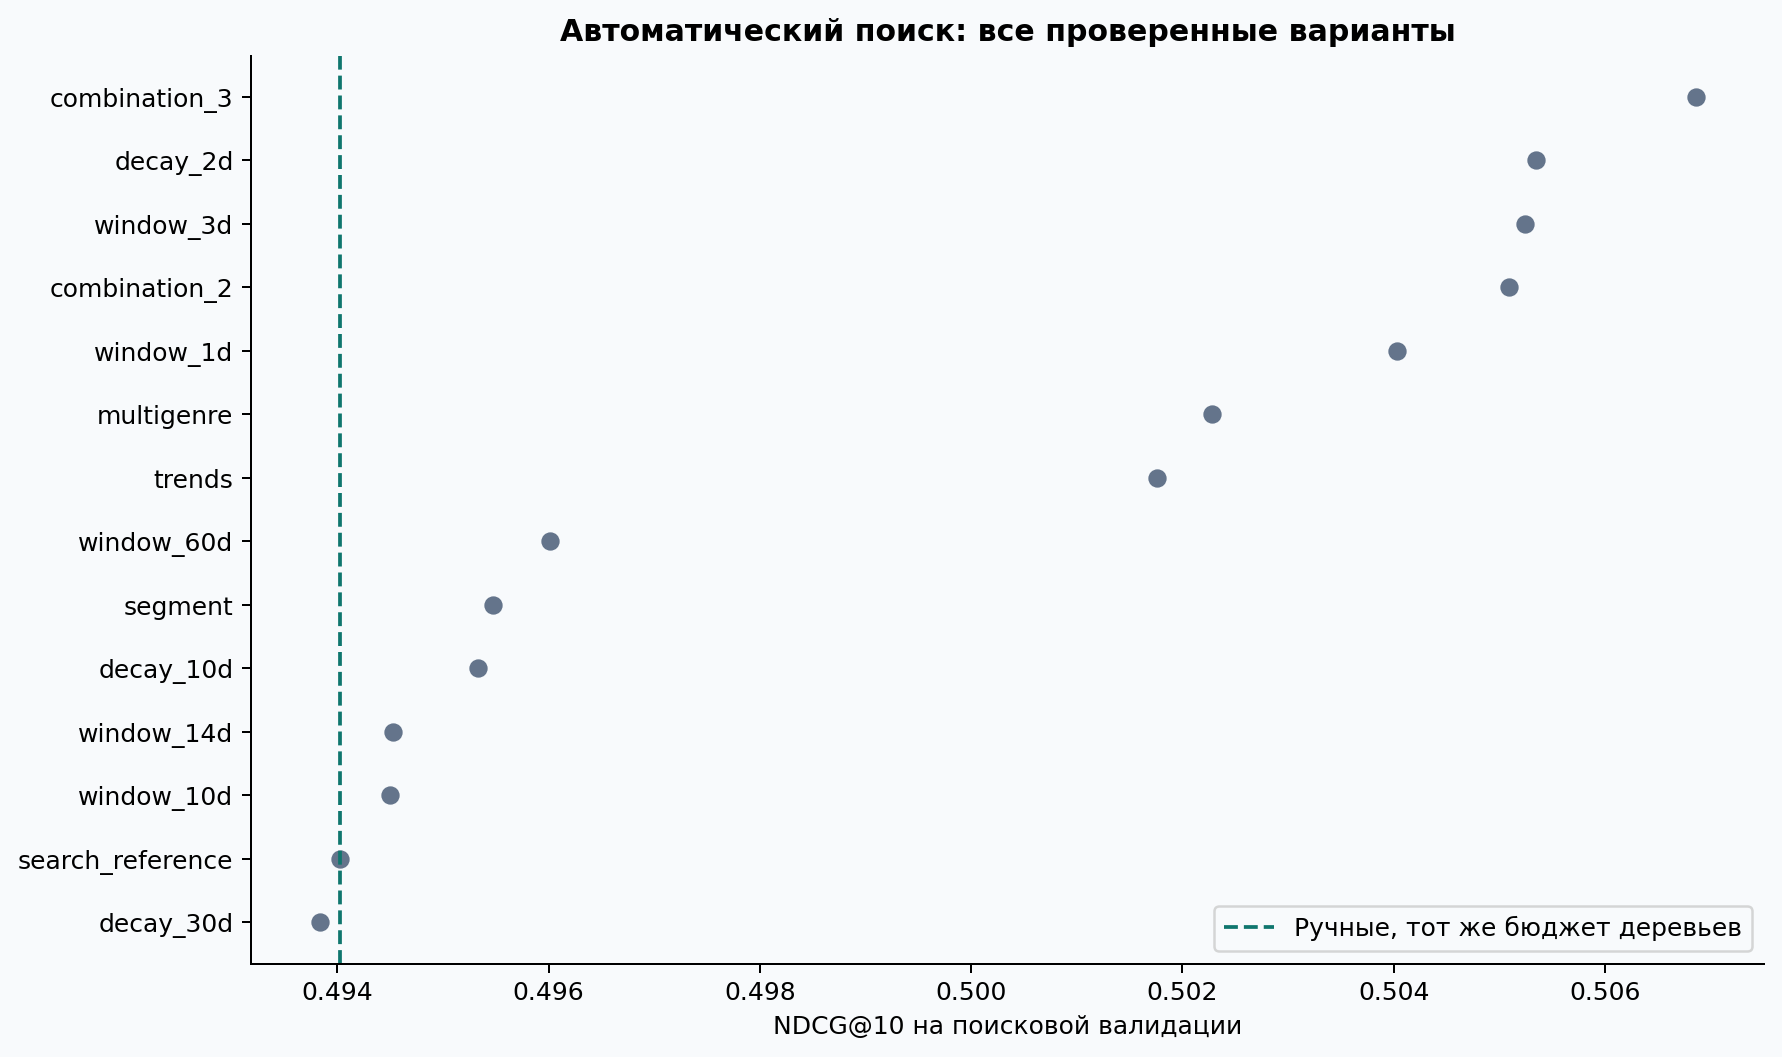
\includegraphics[width=\linewidth,height=.70\textheight,keepaspectratio]{figures/search.png}
\caption{Все результаты автоматического поиска}
\label{fig:search}
\end{figure}
Здесь автоматизируется \textbf{отбор внутри заданного человеком пространства}, а не выбор любых возможных отношений. Более широкий поиск может переобучиться на валидации; отдельный confirm и закрытый test ограничивают этот риск. Вычислительный бюджет поиска превышает бюджет настройки baseline и явно учитывается ниже.

